Recall that the Riemann surface was introduced to better understand the function $y = (1 - x^3)^{1/3}$. Thus one thing we may want to do is check how this function acts on closed curves. Of course this function is multivalued on the complex plane so we will instead try to understand this behaviour by ``pulling back'' to the Riemann surface.

Suppose $\gamma$ is a closed curve in $\C$ that encloses (the images of) the three branch points. Then let $\delta$ be a lift of $\gamma$. In other words, $\delta$ is a curve on $X$ such that $\varphi \circ \delta = \gamma$. Notice that $\delta$ itself need not be closed. 
% TODO: Add diagram of encircling all 3 branch points

Since $y = (1 - x^3)^{1/3}$ lifts to the map $(x, y) \mapsto y$ on the Riemann surface $X$, we want to compute 
$$\frac{1}{2\pi i} \int_\delta \frac{dy}{y}$$

Differentiating the defining equation of $X$ we get 
$$3x^2 dx + 3y^2 dy = 0$$
Therefore 
\begin{align*}
    \frac{dy}{y} = \frac{-x^2 dx}{y^3} = \frac{-x^2 dx}{1 - x^3}
\end{align*}
Now we observe the remarkable fact that 
\begin{align*}
    \frac{1}{2\pi i} \int_\delta \frac{dy}{y} &= \frac{1}{2\pi i} \int_\delta \frac{-x^2 }{1 - x^3} dx\\
    &= \frac{1}{2\pi i} \int_\delta \varphi^* \left( \frac{-z^2}{1 - z^3} dz \right)\\
    &= \frac{1}{2\pi i} \int_{\varphi(\delta)} \frac{-z^2}{1 - z^3} dz\\
    &= \frac{1}{2\pi i} \int_\gamma \frac{-z^2}{1 - z^3} dz
\end{align*}
where $\varphi^*$ in the second line is the pullback.

We can use the Residue Theorem to compute the final integral. The poles of the form are exactly the cube roots of 1 and the residues at each of them is $1/3$. Therefore 
\begin{align*}
    \frac{1}{2\pi i} \int_\delta \frac{dy}{y} = \frac{1}{2\pi i} \int_\gamma \frac{-z^2}{1 - z^3} dz = \frac{1}{3} + \frac{1}{3} + \frac{1}{3} = 1
\end{align*}

Since the integral evaluates to an integer, we conclude that the image of $\delta$ under the map is indeed a closed curve (in particular the argument of $y$ changes by exactly $2\pi$). However, it is clear that this only occurs because $\gamma$ encircles all 3 branch points/poles. If $\gamma$ only contained one of the branch points then the argument would change by $2\pi/3$ and with two branch points the argument would change by $4 \pi/3$. In either of these cases, the result would not be a closed curve. This corresponds exactly with the fact that $y = (1 - x^3)^{1/3}$ is multivalued on $\C$. By the above discussion, we can make this single-valued by introducing cuts on $\C$ as in \autoref{fig:riem-surf-cuts}.

\begin{figure}[ht]
    \centering
    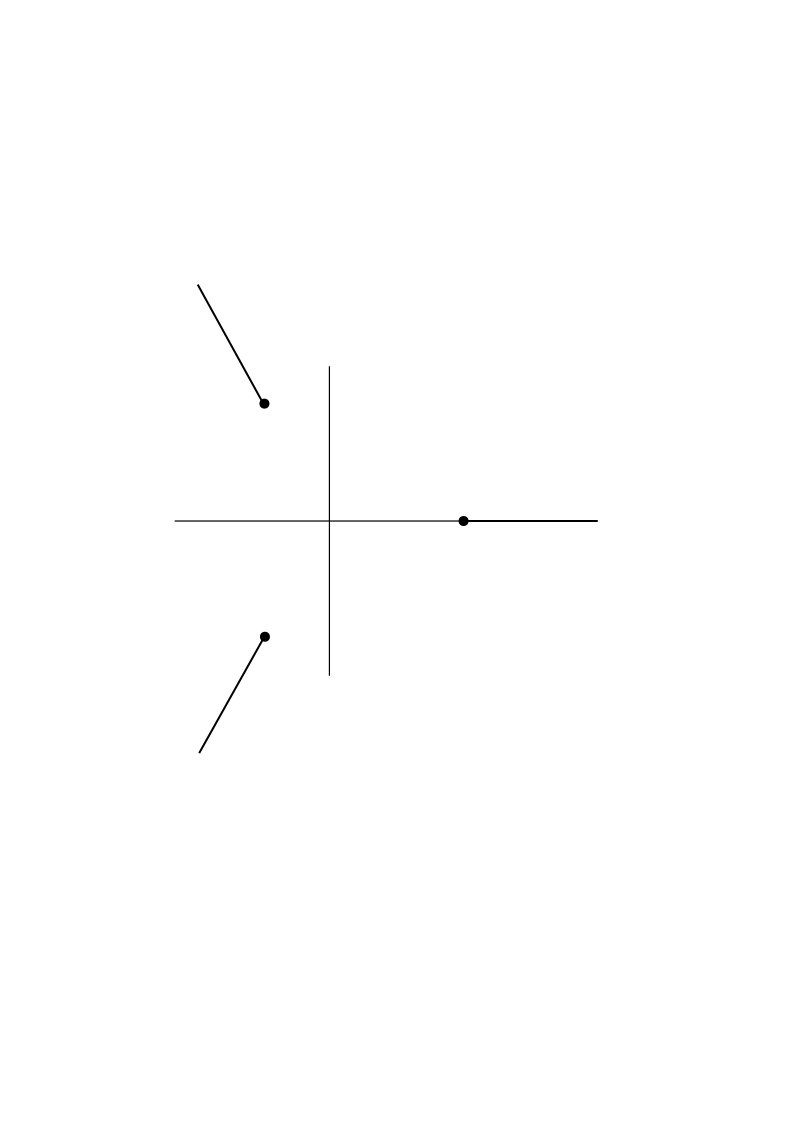
\includegraphics[scale=0.8]{Images/riem_surf_cuts.png}
    \caption{Any closed curve avoiding the cuts either encircles none of the branch points or all of them (remember curves can also extend to $\infty$)}
    \label{fig:riem-surf-cuts}
\end{figure}

By adding these cuts, any closed curve needs to encircle either none or all 3 branch points (if a curve doesn't encircle any of the branch points in one orientation it encircles all of them once the orientation is flipped) which in particular means that the image of any closed curve will be a closed curve. Hence the function $y = (1 - x^3)^{1/3}$ is well-defined. However, we have 3 different choices of the cube root and each choice gives a well-defined holomorphic branch of this function. Therefore the Riemann surface for this function will `look like' 3 copies of the plane with these cuts but these so-called sheets are glued together along these cuts. This is analogous to how the Riemann sphere `looks like' two copies of $\C$ that are glued along $\C \setminus \{0\}$. 

% TODO: Add diagram of the gluing

\begin{remark}
    The cuts made above are somewhat arbitrary. Any choice of cuts that forces closed curves to encircle all 3 branch points is valid.
\end{remark}

% TODO: The cut stuff

% TODO: Complete this section

\subsubsection{Evaluation of a real integral}
One very nice use of the above construction(s) is that it allows us compute real integrals. For example, suppose we want to evaluate 
\begin{align*}
    \int_0^1 \frac{dx}{(1 - x^3)^{1/3}}
\end{align*}

We will do so by viewing this integral in the complex numbers. Of course, the function is multi-valued over $\C$ so we will go to the Riemann surface so that we have a well-defined holomorphic function. 

Since we want to integrate from 0 to 1, we will introduce suitable cuts and integrate along a contour as in \autoref{fig:integral-contour}. 
\begin{figure}[ht]
    \centering
    \includegraphics{Images/integral_contour.png}
    \caption{We introduce cuts from the origin to branch points and integrate just slightly around them}
    \label{fig:integral-contour}
\end{figure}

To be precise, we want to know what happens as we let the countour approach the cut. We can break this integral as the sum of the 6 straight lines (the integrals over the circular arcs have negligible contribution in the limit). However, notice that every time we go around a branch point, the argument of the denominator increases by $2 \pi/3$. For example, let us denote the integral over $\gamma_1$, the integral from 0 to 1, by $I$ (this is what we are trying to evaluate). The integral over $\gamma_2$ is the same integral from 1 to 0 so it should be the same as I except we pick up a negative sign due reversing the orientation and the denominator picks up a factor of $j = e^{2 \pi i/3}$. Thus we have 
\begin{align*}
    \int_{\gamma_1} \frac{dz}{(1 - z^3)^{1/3}} + \int_{\gamma_2} \frac{dz}{(1 - z^3)^{1/3}} = I - \frac{1}{j}I = I - j^2 I
\end{align*}

Now we want to compute the integral over $\gamma_3$. Notice that $\gamma_3(t) = j \cdot \gamma_1(t)$. Moreover, since the denominator picked up a factor of $j$ when going around 1, we have
\begin{align*}
    \int_{\gamma_3} \frac{dz}{(1 - z^3)^{1/3}} = \int_{\gamma_1} \frac{d(jz)}{j(1 - (jz)^3)^{1/3}} = \int_{\gamma_1} \frac{dz}{(1 - z^3)^{1/3}} = I
\end{align*} 

Similarly we get 
$$ \int_{\gamma_4} \frac{dz}{(1 - z^3)^{1/3}} = -j^2 I $$
and of course the same thing will hold for the remaining two curves due to the same reasoning
\begin{align*}
    \int_{\gamma_5} \frac{dz}{(1 - z^3)^{1/3}} &= I\\
    \int_{\gamma_6} \frac{dz}{(1 - z^3)^{1/3}} &= -j^2 I
\end{align*}

Then if we denote the entire contour by $\delta$ we have 
\begin{align*}
    \int_{\delta} \frac{dz}{(1 - z^3)^{1/3}} = 3(I - j^2 I)
\end{align*}

On the other hand, we can also use the Residue Theorem to compute the left hand side. In particular we will use the residue at $\infty$. 

In order to compute the residue at $\infty$, we will simply switch to coordinates at $\infty$ so let $u = 1/x$. Then 
\begin{align*}
    \frac{dx}{(1 - x^3)^{1/3}} = \frac{d(1/u)}{(1 - (1/u)^3)^{1/3}} = -\frac{du}{u^2(1 - 1/u^3)^{1/3}} = - \frac{du}{u(u^3 - 1)^{1/3}}
\end{align*}

The residue of this form at $u = 0$ is $-1/(-1)^{1/3}$. Notice we have 3 different answers corresponding to the three distinct lifts of $\delta$ or the three distinct points at $\infty$. Therefore 
\begin{align*}
    3(I - j^2I) = \int_{\delta} \frac{dz}{(1 - z^3)^{1/3}} = 2\pi i \cdot \{\text{one of } 1, j, j^2\}
\end{align*}

In order to determine what the value of the integral is, we use the fact that $I$ is a real integral and hence the answer should be real. Trying the three different options, we determine that the only possible choice is $j$ which gives 
$$ I = \int_{0}^1 \frac{dx}{(1 - x^3)^{1/3}} = \frac{2\pi}{3 \sqrt{3}} $$


% TODO: Finish integrating section

\subsection{Riemann surfaces and Elliptic Curves}
Suppose we have an equation of the form 
$$y^2 = P(x)$$
where $P$ is a polynomial of degree 3 with 3 distinct roots. Without loss of generality we can assume that the coefficient of $x^2$ is 0 by completion of the cubic (for example if we have $P(x) = x^3 + ax^2 + bx + c$ then we can consider $P(x - a/3)$ which has no quadratic term). Therefore we can write
\begin{equation}\label{eq:ellptc-curve}
    y^2 = 4x^3 - 20a_2x - 28a_4
\end{equation}
where $a_2, a_4$ are just suggestively labeled constants. 

We then get a Riemann surface $\varphi: X \to \C$ where $X$ is the curve defined by the given equation in $\C \times \C$ where $\varphi$ is the projection onto the $x$ coordinate (exactly as we had earlier). We can then complete this to the curve $X' \subset P^2(\C)$. We saw in \autoref{subsec:compact-ellptc-curve} that there is a single point at infinity $[0, 1, 0]$ and the extension $\varphi': X' \to S^2$ is holomorphic at this point.

Consider the form $dz$ which is given by 
\begin{align*}
    \frac{dx}{y}
\end{align*}
when $x$ is a local coordinate (i.e. $y \neq 0$). Computing the differential of both sides of \eqref{eq:ellptc-curve}, we see that 
\begin{align*}
    2ydy = 12x^2 - 20 a_2 dx 
\end{align*}
This means that 
\begin{align*}
    \frac{dx}{y} = \frac{dy}{6x^2 - 10 a_2}
\end{align*}
Therefore when $y$ is a local coordinate (i.e.when $x \neq 0$) we can use the right hand side to evaluate the integral. 

The holomorphic differential form $\omega$ has a local primitive at every point of $X$. Globally the primitive is a multi-valued function given by the integral of $\omega = dx/y$. Notice that any branch of $z$ serves as a coordinate in a neighbourhood of any point of $X$. 

At $[0, 1, 0]$, the chart is given by $[x', 1,t']$ which in our usual coordinates is $[x'/t', 1/t', 1]$ so that $x = x'/t'$ and $y = 1/t'$. Thus 
\begin{align*}
    \omega &= \frac{dx}{y}\\
    &= t' d(x'/t')\\
    &= dx' - \frac{x'}{t'}dt'\\
    &= dx' - x' \cdot \frac{12x'^2 + \cdots}{4x'^3 + \cdots} dx'\\
    &= -2 (1 + g(x')) dx'
\end{align*}
where $g$ is a holomorphic function satisfying $g(0) = 0$. 

Recall from our discussion of $\wp$ that if $\Gamma$ is a discrete group and 
$$a_2 = 3 \sum_{\omega \in \Gamma \setminus \{0\}} 1/\omega^4 \text{ and } a_4 = 5 \sum_{\omega \in \Gamma \setminus \{0\}} 1/\omega^6$$
then the meromorphic transformation $x = \wp(z)$ and $y = \wp'(z)$ induces a biholomorphism $\C/\Gamma \to X'$ given by $z \mapsto [\wp(z), \wp'(z), 1]$. Notice that $dx = \wp'(z)dz = y dz$ so $dz = dx/y$. Thus in particular the inverse of the biholomorphism is given by the multivalued function 
$$z = \int dz = \int \frac{dx}{y} = \int \omega $$
The branches of $z$ differ by the constants in $\Gamma$. Abel's Theorem below tells us that this result has something of a converse. Namely given an elliptic curve, we can recover the discrete group.

\begin{theorem}[Abel's Theorem]
    Suppose we are given constants $a_2, a_4$ such that $P(x) = 4x^3 - 20a_2 x - 28 a_4$ has 3 distinct roots. Then there exists a discrete group $\Gamma$ such that $a_2 = 3 \sum 1/\omega^4$ and $a_4 = 5 \sum 1/\omega^6$. It follows that $y^2 = P(x)$ has a parameterisation given by $x = \wp(z)$ and $y = \wp'(z)$. 
\end{theorem}

We will give a sketch of the proof as the complete proof requires some algebraic topology and other results. The proof requires 2 lemmas.

\begin{lemma}
    Let $z = \int \omega = \int dy/x$ by the multivalued function arising from the curve $y^2 = P(x)$. Then branches of $z$ differ from each other by constants that form a discrete group $\Gamma$ of $\C$ where $\Gamma$ is generated by two complex numbers $e_2$ and $e_2$ which are linearly independent over $\R$. 
\end{lemma}
\begin{proof}
    Notice that $z = \int \omega$ is well definied up to the addition of a period, i.e. up to the addition of $\int_\gamma w$ where $\gamma$ is a $C^1$ closed curve (technically a a 1-cycle or a 1-chain with 0 boundary) in $X'$. If $\gamma$ is the boundary of a 2-chain, then $\pi(\gamma) = \int_\gamma \omega = 0$ by Stokes' Theorem. 

    Then $\pi$ induces a homomorphism from the first homology group $H_1(X, \Z)$ to $\C$. Thus $z: X' \to \C/\Gamma$ where $\Gamma = \{\pi(\gamma) : \gamma \in H_1(X', \Z)\}$ is the group of periods. By the Riemann-Hurwitz formula, we compute that $H_1(X', \Z) = \Z \oplus \Z$. In particular then $\Gamma$ is generated by two complex numbers $e_1$ and $e_2$. They are either linearly independent over the reals or they are not. If they are then we get a lattice as claimed. If not then $\Gamma$ is contained in a 1-dimensional subspace of $\C$. We show this cannot happen.

    Suppose $\Gamma$ is contained in a 1-dimensional subspace of $\C$. Then by applying an appropriate rotation, i.e. by multiplying by an appropariate unit complex number $\alpha$ we get that $\alpha \Gamma$ is contained in the imaginary axis. In particular then $\Re(\alpha \pi(\gamma))$ for all $\gamma \in H_1(X', \Z)$ is 0. Recall we argued above that the branches of $z$ can only differ by an element of $\Gamma$. Therefore if $\Re(\alpha \pi(\gamma))$ is 0 for all $\gamma$ then $\Re(\alpha z)$ is a (single-valued) harmonic function on $X'$. Since $X'$ is a compact, the function attains a maximum. But then by the maximum modulus principle we conclude that $\Re(\alpha z)$ is constant. Since a holomorphic function is constant if and only if its real part is constant, this would imply that $z$ is constant, leading to a contradiciton. 

    \begin{figure}[ht]
        \centering
        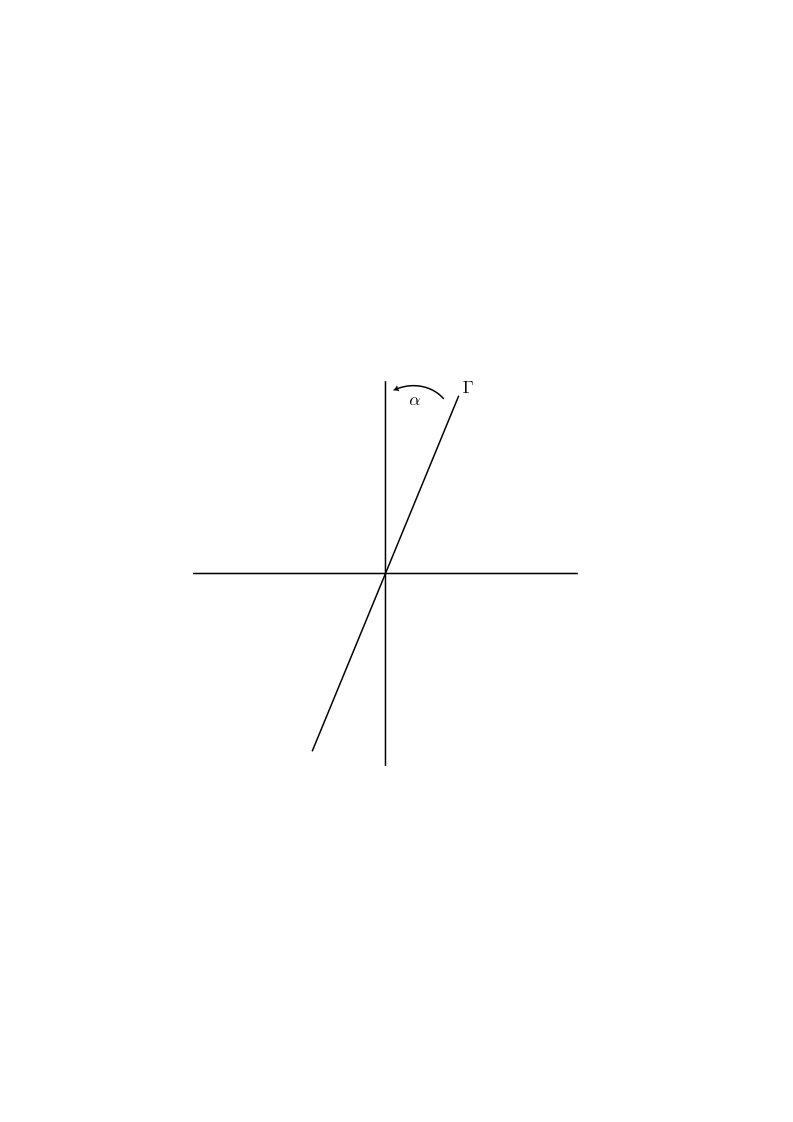
\includegraphics[scale=0.8]{Images/Gamma_in_1_dim_space.png}
        \caption{If $\Gamma$ is contained in a 1-dimensional subspace, we can rotate it to be contained in the imaginary axis}
        \label{fig:Gamma-in-1-dim-subspace}
    \end{figure}
\end{proof}

Now that we have found a lattice we want to show that this lattice gives rise to the same elliptic curve.

\begin{lemma}
    The map $X' \to \C/\Gamma$ given by 
    $$z(p) = \int_{p_0}^p \omega$$
    (where $p_0$ is the point at infinity $[0, 1, 0]$) is a biholomorphism and in fact the composition
    \begin{align*}
        X' &\to \C/\Gamma \to X''\\
        p &\mapsto z \mapsto [\wp(z), \wp'(z), 1]
    \end{align*}
    is the identity.
\end{lemma}
\begin{proof}
    The first part of the lemma about $z$ being a biholomorphism requires some algebraic topology so we will simply believe it.

    Notice that $x$ is a meromorphic function on $X'$ with a pole of order 2 at $p_0 := [0, 1, 0]$. This follows from work we've done previously. 
    The coordinates near $\infty$ of $X'$ are given by $[x', 1, t']$ where we know from \autoref{subsec:compact-ellptc-curve} that 
    $$t' = 4x'^3 - 320a_2 x'^7 + \cdots$$
    In our usual $[x, y, 1]$ coordinates then we have 
    \begin{align*}
        x = \frac{x'}{t'} = \frac{x'}{4x'^3 - 320a_2 x'^7 + \cdots}
    \end{align*}

    Then via the biholomorphism $z$, we can pull back $x$ to a function on $\C/\Gamma$. Since $z$ maps $p_0$ to 0, we know that $x$ has a pole of order 2 at $z = 0$. Therefore 
    \begin{align*}
        x(z) &= \frac{c}{z^2} + \frac{d}{z} + e + fz + \cdots \\
        x'(z) &= -\frac{2c}{z^3} - \frac{d}{z^2} + f + \cdots
    \end{align*}
    Then since $dz = dx/y$ we have $x'(z) = y$. Therefore 
    \begin{align*}
        x'(z)^2 = y^2 = 4x^3 - 20a_2 x - 28a_4
    \end{align*}
    Substituting the above series and equating coefficients we conclude that $c = 1$, $d = 0$ and $e = 0$. This means that $x(z)$ and $\wp(z)$ (with respect to the lattice $\Gamma$) have the same principal part so $x(z) - \wp(z)$ is a doubly periodic, entire function so must be constant. Since the difference is 0 at 0, we conclude that $x(z) = \wp(z)$ everywhere.
\end{proof}